\chapter{Introduction}
\label{ch:introduction}

The source code, workflow definitions, and configuration files of this study are publicly available in the \href{https://github.com/thealanjason/mcmc-bench}{\texttt{mcmc-bench} GitHub repository}.

Computational models are widely used to represent and predict the behaviour of complex systems, but their predictions often depend on input parameters whose values are unknown for the application under study. Model calibration uses observations of the physical system to learn about these unknown inputs by adjusting the corresponding model parameters. This connection between observations and model parameters is important not only for improving predictive performance, but also for representing the uncertainty that remains after calibration and accounting for discrepancies between the simulator and reality \autocite{Kennedy2001}.

Bayesian inference provides a formal framework for \emph{learning from experience}. Existing knowledge or assumptions about unknown quantities are represented by a prior distribution, while observations enter the analysis through the likelihood. Combining these two sources of information produces the posterior distribution, which expresses what has been learned after observing the data \autocite{Zyphur2015}. This principle is not restricted to a particular application area; Bayesian methods are widely used to reason about uncertain parameters and predictions across a broad range of scientific disciplines \autocite{vanDeSchoot2021}. In model calibration, the posterior therefore describes which parameter values remain plausible after seeing the model with observations, rather than returning only a single fitted value \autocite{Kennedy2001}.

All of the model parameters do not have the same interpretation. Physical parameters have meaning within the scientific description of a system, although their values may be unknown or difficult to measure directly from the physical system. On the other hand, tuning parameters have no direct physical interpretation; they are often introduced as simplified representations of processes that the simulator does not explicitly resolve and are adjusted to improve agreement with observations \autocite{Brynjarsdottir2014}. This distinction affects how calibration results should be interpreted: learning about a physical parameter may provide information about the system, whereas an inferred tuning parameter remains specific to the model. In the Voellmy model considered here, $\mu$ and $\xi$ enter the resistance law as dry-Coulomb and turbulent friction coefficients, respectively. However, they are effective, conceptual parameters rather than directly measurable material constants, and their values are commonly inferred by back-analysing observed events from the field data \autocite{Heredia2020,Yildiz2023}.

Bayesian calibration typically requires repeated evaluations of the forward model, which might be expensive. A statistical emulator can be used to approximate the simulator outputs from a smaller set of precomputed runs; RobustGaSP provides Gaussian-process emulators for this purpose \autocite{Gu2024,Yildiz2023}. The benchmark in this report therefore operates on an existing RobustGaSP surrogate of the gravity-driven mass flow model rather than executing the full simulator during sampling. All integrated samplers use this same surrogate model and target the same sampler-agnostic posterior. Here, sampler-agnostic means that the prior and likelihood, and therefore the mathematical target distribution, are defined independently of the sampling algorithm. The benchmark can thus evaluate how accurately and efficiently each method approximates the same target, while recognizing that finite-run and implementation effects may still produce different numerical results.

%%%%%%%%%%%%%%%%%%%%%%%%%%%%%%%%%%%%%%%%%%%%%%%%%%%%%%%%%%%%%%%%%%%%%%%%
\section{Motivation}
\label{sec:motivation}

Gravity-driven mass flow models simulate the runout of avalanches, debris flows, and related flow-like landslides, providing estimates of quantities such as flow depth, velocity, and impact area. These outputs points hazard maps and quantitative risk assessments and can inform mitigation planning and model-based decision support \autocite{Yildiz2023}. Their practical value, however, depends on the reliability of the simulated event behaviour. Because the effective resistance parameters cannot  be measured directly, they must be calibrated against observations, and the uncertainty associated with this calibration must be considered when interpreting model predictions \autocite{Heredia2020,Yildiz2023}.

\begin{figure}[tbp]
  \centering
  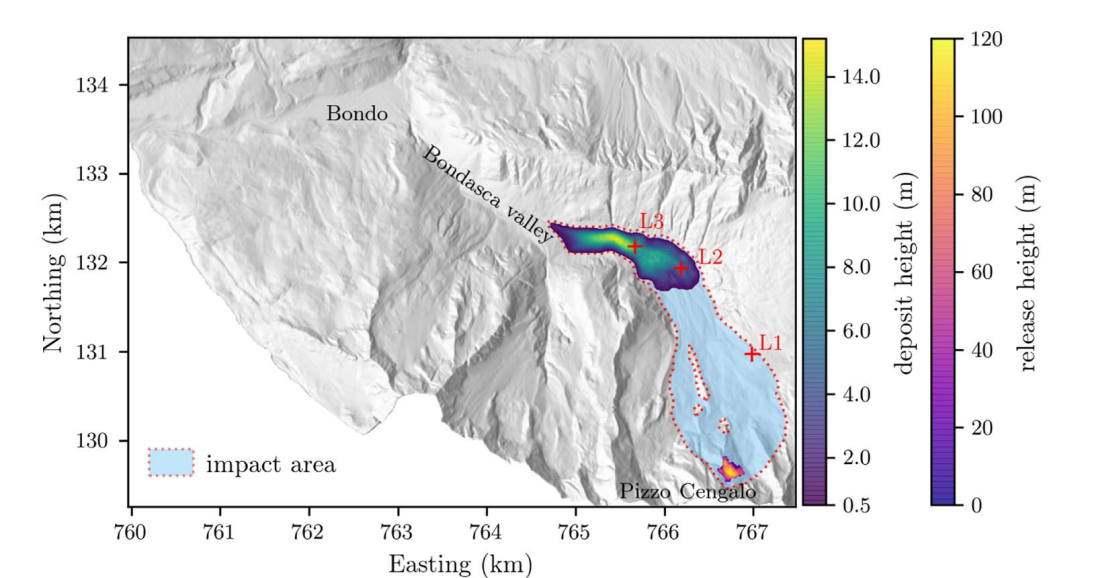
\includegraphics[width=\textwidth]{images/kowalski-topography-mass-dsstribution-bondo-landslide.png}
  \caption{Topography and release mass distribution of the 2017 Bondo landslide, together with the simulated impact area and deposit distribution for Voellmy parameters $\mu = 0.23$ and $\xi = 1000\,\mathrm{m\,s^{-2}}$. Reproduced without modification from \textcite[Fig.~2]{ZhaoKowalski2022} under the \href{https://creativecommons.org/licenses/by/4.0/}{CC BY 4.0 license}.}
  \label{fig:bondo-topography}
\end{figure}

A deterministic calibration can be formulated as an optimization problem that returns a parameter vector minimizing the discrepancy between model outputs and observations. However, observations contain measurement error. If these sources of error are not represented explicitly, the fitted parameters may include noise leading to biased conclusions \autocite{Kennedy2001,Brynjarsdottir2014}. Calibration may also suffer from identifiability problems: different parameter combinations, or different allocations between parameters and model discrepancy, can explain the observations similarly well \autocite{Arendt2012}. Consequently, a single best point does not account for the result. The relevant question is instead: \emph{which combinations of parameter values are supported by the observations, and how is uncertainty distributed across those combinations?}

Bayesian calibration addresses this problem by representing uncertainty about model parameters through a posterior distribution rather than a single estimate. The prior has assumptions before observing the calibration data, while the likelihood describes how the observations relate to model outputs; together they define the posterior on the selected model and data \autocite{Kennedy2001}. Reliable predictive uncertainty quantification also requires consideration of model discrepancy and surrogate uncertainty \autocite{Brynjarsdottir2014,Yildiz2023}. Such study is not evaluated in this benchmark; here, the posterior serves as the common target distribution for all of the samplers.

When posterior quantities cannot be computed analytically, sampling algorithms are used to explore the target distribution \autocite[Sections~1--2]{Albert2025}. These samplers differ in how they handle challenging posterior geometries, and their relative accuracy and efficiency can depend on the structure of the target distribution and on implementation details \autocite[Abstract and Sections~1 and~4.1]{Albert2025}.

The samplers currently integrated into the benchmark use different Python packages and run in sampler-specific software environments. However, the \texttt{mcmc-bench} repository implements a modular and extensible benchmarking framework rather than a Python-only sampler interface. Its execution is orchestrated as a Nextflow workflow, while UM-Bridge exposes the surrogate through a language-agnostic model interface. This separation allows future sampling methods implemented in other programming languages to be integrated without modifying the model interface \autocite[Summary and Statement of Need]{Seelinger2023}. For the current comparison, all samplers are configured to use the same surrogate, prior, and likelihood, which together define the common sampler-agnostic posterior.

%%%%%%%%%%%%%%%%%%%%%%%%%%%%%%%%%%%%%%%%%%%%%%%%%%%%%%%%%%%%%%%%%%%%%%%%
\section{Research Questions}
\label{sec:research-questions}

Our research questions are as follows:
\begin{itemize}
  \item[\textit{RQ1}] How can different sampling methods be integrated into a modular, extensible, and reusable framework for Bayesian calibration of a surrogate-based gravity-driven mass flow model?

  \item[\textit{RQ2}]
  Which accuracy, convergence, and computational-efficiency criteria enable a meaningful comparison of the integrated sampling methods, and how do the samplers perform according to these criteria in the Voellmy calibration case study?
\end{itemize}

%%%%%%%%%%%%%%%%%%%%%%%%%%%%%%%%%%%%%%%%%%%%%%%%%%%%%%%%%%%%%%%%%%%%%%%%
\section{Outline}
\label{sec:outline}

The followings of this report are organized as follows. Chapter~\ref{ch:relatedwork} introduces inverse problems, Bayesian calibration, surrogate modeling, and the selected sampling methods. Chapter~\ref{ch:ownwork} describes the common benchmarking framework and the integration of the five samplers. Chapter~\ref{ch:evaluation} presents the experimental setup, comparison criteria, results, and discussion. Finally, Chapter~\ref{ch:summary} summarizes the findings and outlines future work.

